\subsection{Testversion}
\label{kap:McpExecutorTestversion}
Um die Funktionen der Chips zu verstehen und beherrschen zu können erfolgt der Aufbau einer Einheit auf einem Entwicklungsboard (Whiteboard). Dieser Aufbau beinhaltet alles, was für eine Einheit vorgesehen ist, d.h. einen Atmega328 (mit externem Taktgeber), einen Adxl345 und einen Mcp2515. Mit entsprechender Verdrahtung (s. Schaltbild \ref{fig:SchaltbildEinheit}) und der Entwicklung eines Programms, welches auf der MCU aktiv ist, lassen sich die Sensorwerte über einen CAN-Bus auslesen. Die Sensor-ID muss programmatisch auf der MCU definiert werden. 

\begin{figure}[H]
	\centering
	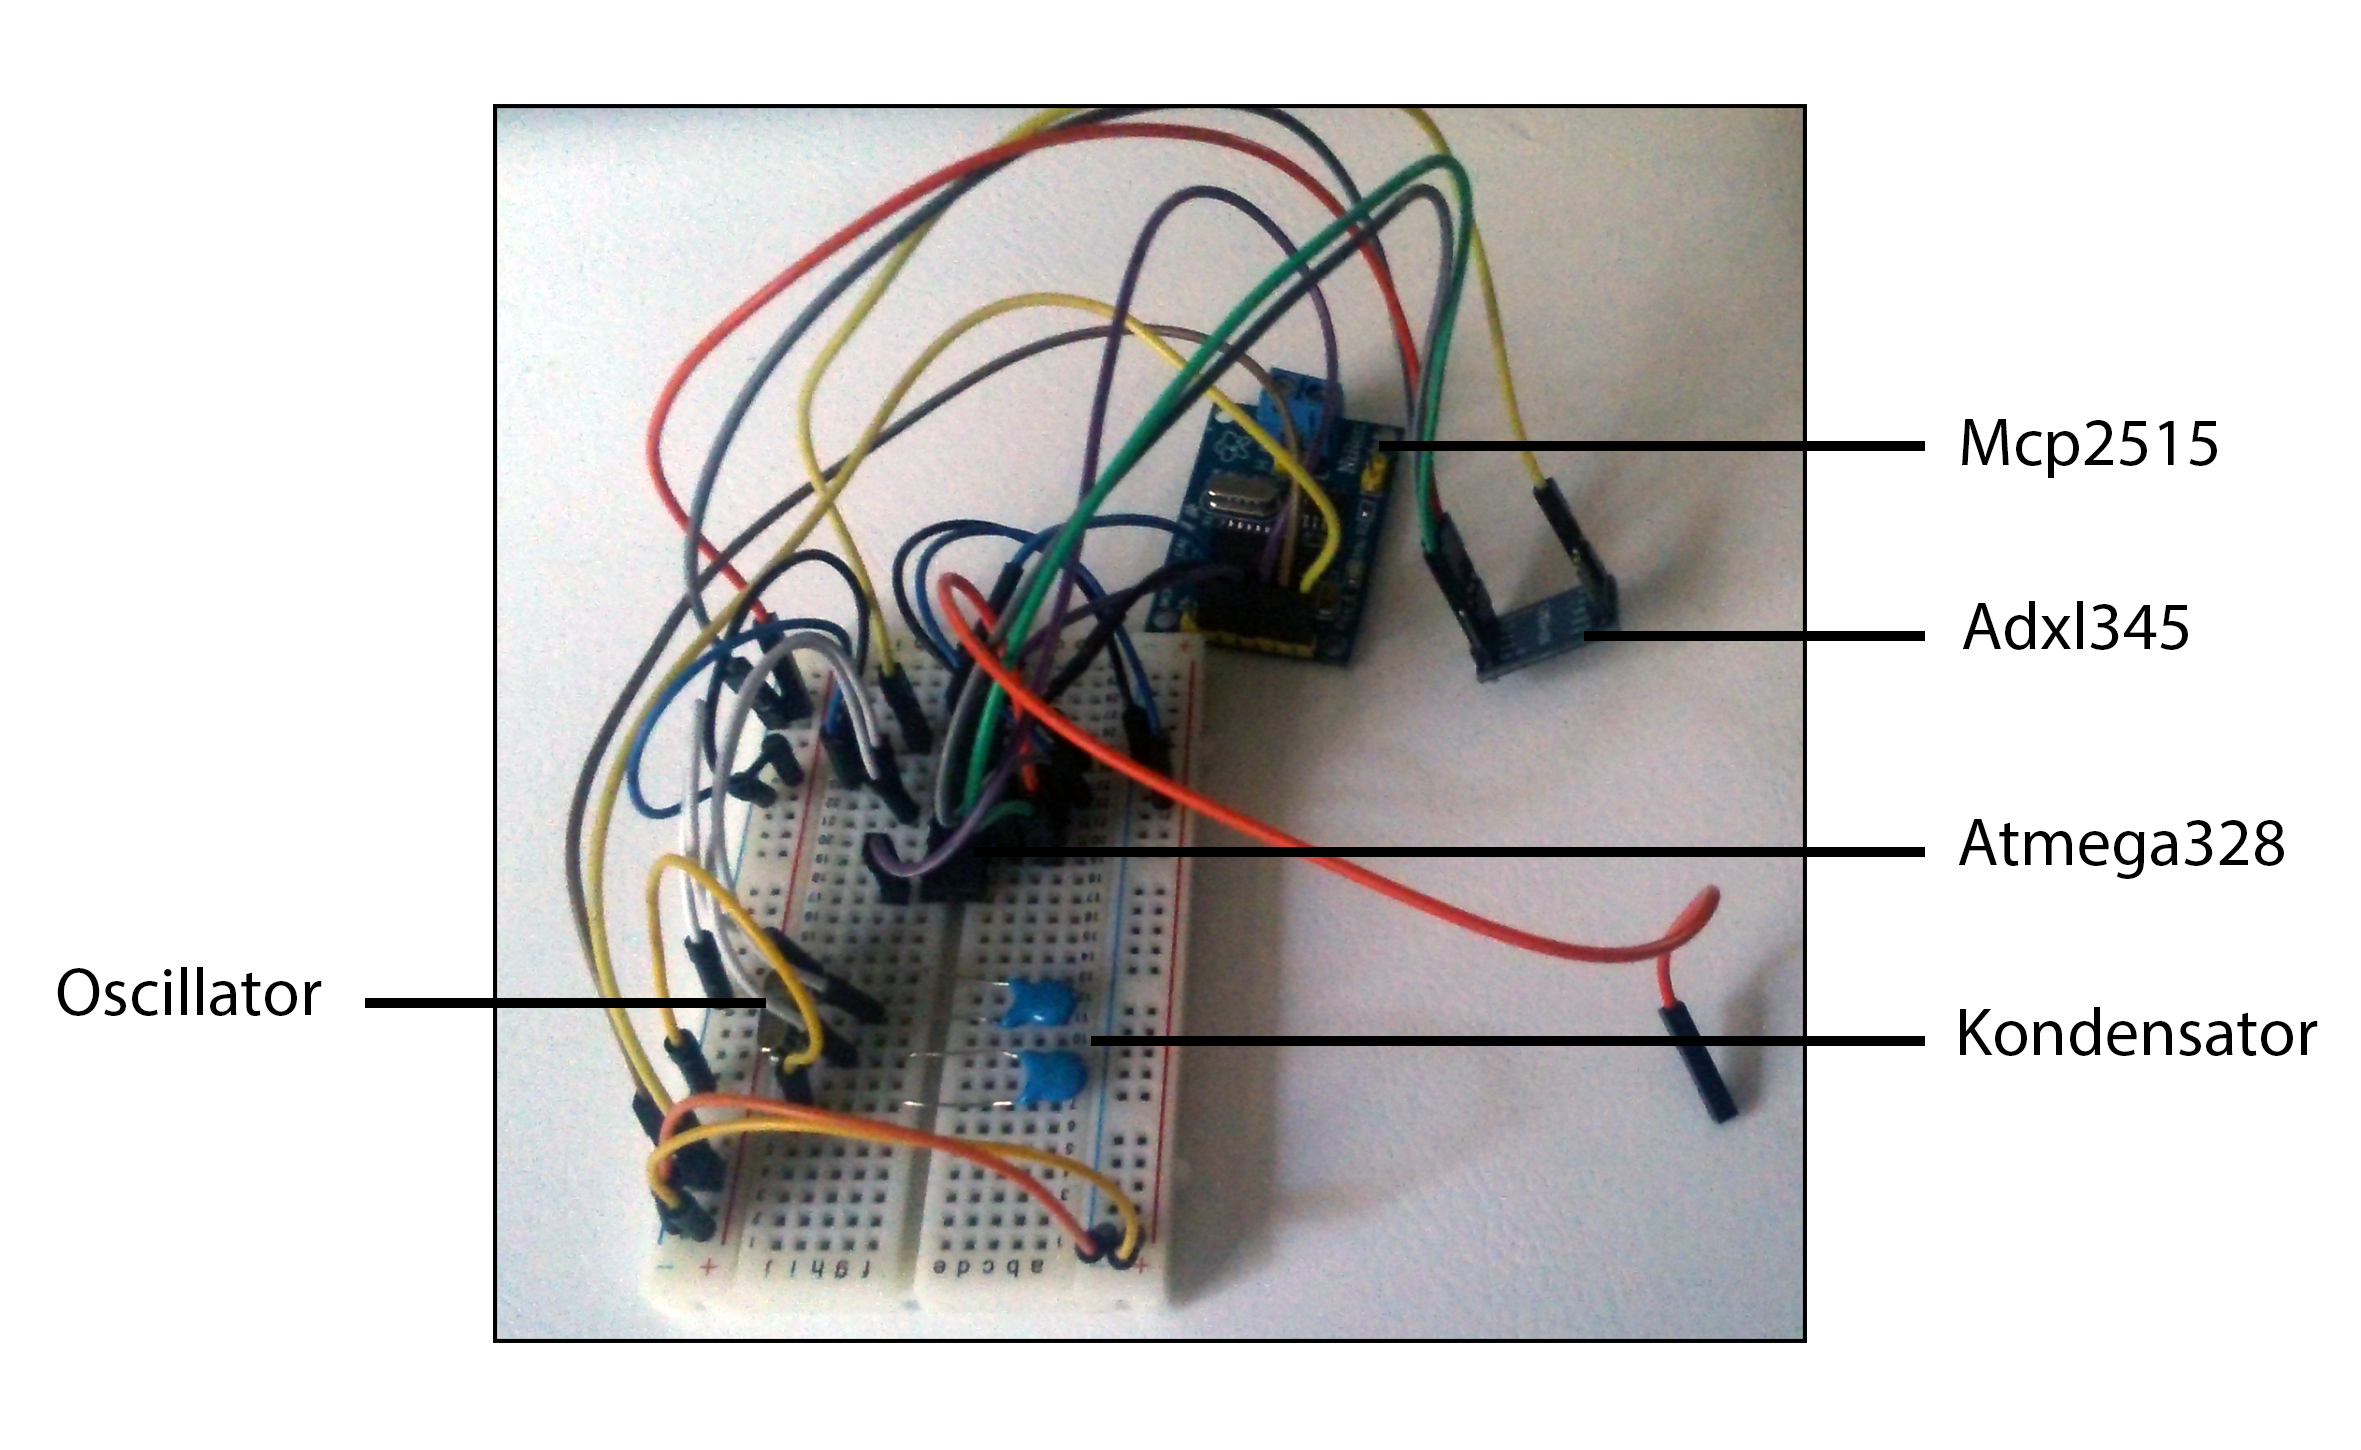
\includegraphics[width=0.9\linewidth]{Bilder/McpExecutorTest}
	\caption[Testversion einer Mcp-Executor-Einheit]{Testversion einer Mcp-Executor-Einheit}
	\label{fig:McpExecutorTest}
\end{figure}

Mit zwei solcher Testaufbauten wurde das Aufnehmen von Sensorwerten validiert.